%----------------------------------------------------------------------------------------
%	PACKAGES AND THEMES
%----------------------------------------------------------------------------------------
\PassOptionsToPackage{table}{xcolor}
\documentclass[aspectratio=169,xcolor=dvipsnames,11pt]{beamer}
\usetheme{SimplePlusAIC}
\usepackage{amsmath}
\usepackage{animate}
\usepackage{hyperref}
\usepackage{cleveref}
\usepackage{caption}
\usepackage{graphicx} % Allows including images
%\usepackage{subfig}
\usepackage{subcaption}
\usepackage{booktabs} % Allows the use of \toprule, \midrule and  \bottomrule in tables
\usepackage{svg} %allows using svg figures
\usepackage{tikz}
\usetikzlibrary{intersections}
\usepackage{makecell}
\usepackage{multirow}
\usepackage{appendixnumberbeamer}
\usepackage{wrapfig}
\usepackage{verbatim}
\usepackage{tcolorbox}
%\usepackage[dvipsnames]{xcolor}

\usepackage{hhline}
\usepackage{relsize}
\usepackage{bm}
%Select the Epilogue font (requires luaLatex or XeLaTex compilers)
%\setsansfont{Epilogue}[
  %  Path=./epilogueFont/,
  %  Scale=0.9,
  %  Extension = .ttf,
   % UprightFont=*-Regular,
   % BoldFont=*-Bold,
   % ItalicFont=*-Italic,
    %BoldItalicFont=*-BoldItalic
    %]
    \usefonttheme[onlymath]{serif}
% \usepackage{ eulervm } % Euler VM as math serif font

\newcommand*{\defeq}{\stackrel{\text{def}}{=}}
\newcommand{\grad}{\nabla}
\newcommand{\lap}{\Delta}
\newcommand{\weaklyto}{\rightharpoonup}
\newcommand{\weakstar}{\stackrel{*}\rightharpoonup}
\newcommand{\cts}{\hookrightarrow}
\newcommand{\ctsDense}{\xhookrightarrow{d}}
\newcommand{\ctsCompact}{\xhookrightarrow{c}}
\newcommand{\E}{\mathbb{E}}
\newcommand{\pP}{\mathbb{P}}
\newcommand{\R}{\mathbb{R}}
\newcommand{\ER}{\overline{\mathbb{R}}}
\newcommand{\cR}{\mathcal{R}}
\newcommand{\cJ}{\mathcal{J}}
\newcommand{\cG}{\mathcal{G}}
\newcommand{\CVaR}{\textup{CVaR}}
\newcommand{\D}{\textup{ d}}
\newcommand{\dd}{\mathrm{d}}
\newcommand{\fa}{\text{for all }}
\DeclareMathOperator*{\essinf}{\vphantom{p}ess\,inf}
\DeclareMathOperator{\sigmoid}{expit} % a.k.a. logistic sigmoid

\usepackage[ruled,vlined,algo2e]{algorithm2e}
\crefname{algocf}{algorithm}{algorithms}
 \usepackage{caption}

\usepackage{tcolorbox}  % For fancy boxes
\usepackage{lipsum}     % For dummy text

% Define a custom style for the box
\tcbuselibrary{skins, breakable}
\newtcolorbox[auto counter, number within=section]{roundedshadowbox}[2][]{
    colback=white, % Background color (kept white)
    colframe=black, % Border color
    boxrule=0.5pt, % Border thickness
    arc=5mm, % Rounded corners
    shadow=true, % Drop shadow effect
    width=\linewidth, % Full width box
    title=#2, % Title text
    #1 % Additional options (e.g., width override)
}

\usepackage{pgfplots}
\pgfplotsset{compat=1.18}

%\PassOptionsToPackage{table}{xcolor}
%\documentclass[aspectratio=169,xcolor=dvipsnames,11pt]{beamer}
%\usetheme{SimplePlusAIC}
%\usepackage{amsmath}
%\usepackage{hyperref}
%\usepackage{cleveref}
%\usepackage{caption}
%\usepackage{graphicx} % Allows including images
%\usepackage{subcaption}
%\usepackage{booktabs} % Allows the use of \toprule, \midrule and  \bottomrule in tables
%\usepackage{svg} %allows using svg figures
%\usepackage{tikz}
%
%\usepackage{pgfplots}
%\pgfplotsset{compat=1.18}
%
%\usepackage{makecell}
%\usepackage{multirow}
%\usepackage{appendixnumberbeamer}
%\usepackage{wrapfig}
%\usepackage{verbatim}
%\usepackage{tcolorbox}
%\usepackage{hhline}
%\usepackage{relsize}
%\usepackage{bm}
%
%\usefonttheme[onlymath]{serif}
%    
\newcommand{\C}{\mathbb C}

%
%%\font\nullfont=cmr10
%
%\usepackage{tcolorbox}  % For fancy boxes
%\usepackage{lipsum}     % For dummy text
%
%% Define a custom style for the box
%\tcbuselibrary{skins, breakable}
%\newtcolorbox[auto counter, number within=section]{roundedshadowbox}[2][]{
%    colback=white, % Background color (kept white)
%    colframe=black, % Border color
%    boxrule=0.5pt, % Border thickness
%    arc=5mm, % Rounded corners
%    shadow=true, % Drop shadow effect
%    width=\linewidth, % Full width box
%    title=#2, % Title text
%    #1 % Additional options (e.g., width override)
%}


%----------------------------------------------------------------------------------------
%	TITLE PAGE
%----------------------------------------------------------------------------------------

\title[\quad\quad\quad LVPP Course II]{The Latent Variable Proximal Point Method II: Derivation, Analysis, and First Numerical Experiments
 } % The short title appears at the bottom of every slide, the full title is only on the title page
%\subtitle{Subtitle}

\author{\small{\bf Thomas M. Surowiec}}

\institute[T.M. Surowiec]{Department of Numerical Analysis and Scientific Computing \newline Simula Research Laboratory \newline Oslo, Norway}
% Your institution as it will appear on the bottom of every slide, maybe shorthand to save space


\date[EMS School]{ {\footnotesize 
K\'acov, Czechia, 15-20 June 2025}}
%----------------------------------------------------------------------------------------
%	PRESENTATION SLIDES
%----------------------------------------------------------------------------------------

\begin{document}

\begin{frame}[plain]
%\setbeamertemplate{footline}{}
\titlepage
\end{frame}

\begin{frame}{Overview}
\tableofcontents
\end{frame}

\section{Penalty and Approximation Methods}
% \begin{frame}\frametitle{Frame Title}
%    \begin{enumerate}
%    	\item Quadratic Penalty
%		\begin{enumerate}
%			\item Definition
%			\item Connection to Moreau-Yosida regularization
%			\item Asymptotic convergence
%			\item Advantages/Disadvantages
%			\item Path-following
%		\end{enumerate}
%	\item Barrier Penalty
%		\begin{enumerate}
%			\item Definition
%			\item Outer vs. Inner approximation
%			\item Primal-dual formulation
%			\item PD does not force $u$ to be nonnegative, this has to be done with careful line search
%		\end{enumerate}
%	\item Augmented Lagrangian (Ito, Kunisch 1990)
%		\begin{enumerate}
%			\item Definition
%			\item A dual-adaptive quadratic penalty scheme, roots in proximal point (Rockafellar)
%			\item For computation, we need $\lambda$ to have a pointwise interpretation, but this may not be guaranteed
%			\item This forces $r \to +\infty$ (as opposed to finite dimensions)
%		\end{enumerate}
%    \end{enumerate}
% \end{frame}
 
 \begin{frame}\frametitle{A Mathematical Fruitfly} 
  \begin{beamercolorbox}[rounded=true, shadow=true, wd=\textwidth]{block title}\centering
  In order to make a nuanced comparison between several methods, we introduce each method using the obstacle problem.
  The methods themselves are widely applicable.
  \end{beamercolorbox}\hfill
  
\visible<2->{
\begin{minipage}{0.7\linewidth}
\begin{beamercolorbox}[rounded=true, shadow=true, wd=\textwidth]{block body}
 We seek a minimizer $u$ of the objective functional:
 \begin{equation*}
 	J(v)
 	=
 	\frac{1}{2}
 	\int_\Omega |\nabla v|^2 \dd x
 	-
 	\int_\Omega f v\dd x
 	\,,
 \end{equation*}
 over
 \[
 K = \{ v \in H^1_0(\Omega) \mid  v \ge \varphi \text{~a.e. }  \}.
 \] 
 Here, $f \in L^2(\Omega)$ and  $\varphi \in H^1(\Omega)$, $\varphi|_{\Gamma} \le 0$.
\end{beamercolorbox}
\end{minipage}%
\begin{minipage}{0.3\linewidth}
 \centering
\begin{figure}
	\centering
	\begin{tikzpicture}
		\node at (-4.2,1.2) {\scriptsize 
	    	$u$};
		\node at (-3.35,0) {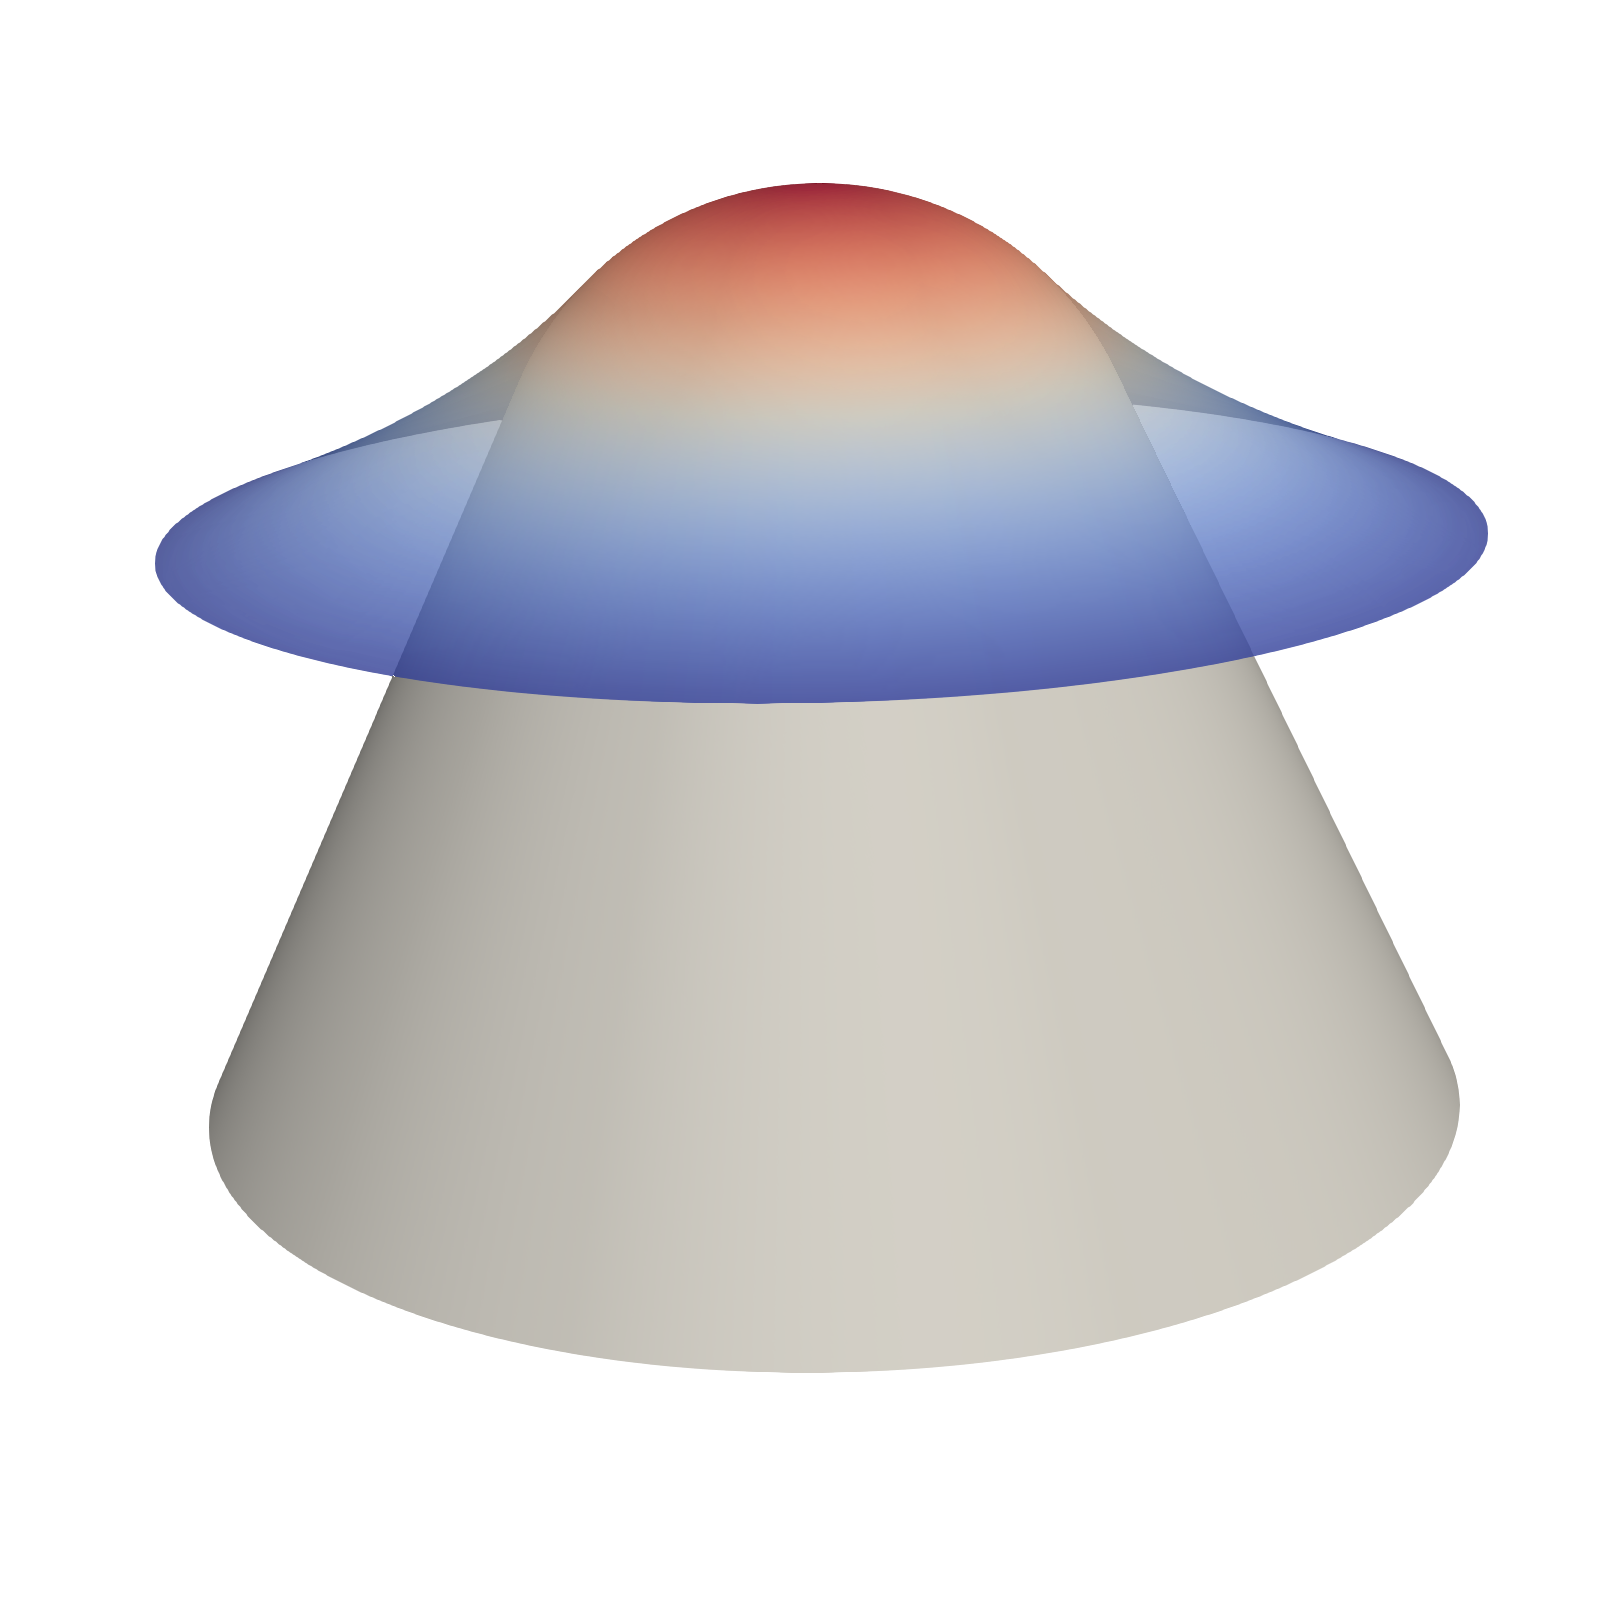
\includegraphics[height=1.25in]{../Part I/figures/obstacle_new.png}};
		\node at (-2.2,-1.35) {\scriptsize 
	    	$\varphi$};
    \end{tikzpicture}
\end{figure}
\end{minipage}}
 \end{frame}
 
 \begin{frame}\frametitle{Penalty Methods}
   \begin{beamercolorbox}[rounded=true, shadow=true, wd=\textwidth]{block body}
This approach involves relaxing the constraints with a smooth penalty function $\beta : V \to \mathbb R$, where $\beta$ is usually convex, $C^{1,1}$ and ideally satisfies
\[
\beta(u) = 0 \text{ if } u \in K\quad \text{ and }\quad \beta(u) > 0 \text{ otherwise. }
\]
  \end{beamercolorbox}
%\begin{minipage}{\textwidth}
% \centering 
 \begin{figure}
% \resizebox{0.3\textwidth}{0.25\textwidth}{%
  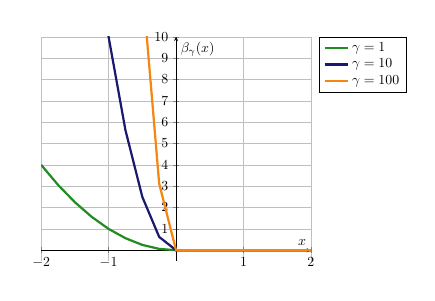
\begin{tikzpicture}[scale=0.5]
    \begin{axis}[
        axis lines=middle, % Draw axes through the origin
        xlabel=$x$,
        ylabel=$\beta_\gamma(x)$,
        xmin=-2, xmax=2, % Adjust x-range as needed
        ymin=-0.5, ymax=10, % Adjust y-range as needed
        grid=both, % Add a grid
        grid style={line width=.1pt, draw=gray!10}, % Style the grid lines
        major grid style={line width=.2pt,draw=gray!50}, % Style major grid lines
        xtick distance=1, % Tick marks every 1 unit on x-axis
        ytick distance=1, % Tick marks every 1 unit on y-axis
        % Add a legend
        legend pos=outer north east, % Position the legend
        legend cell align=left,
        no markers, % Don't put markers on the plots
    ]

    % Define the function with a placeholder for c
    % We use 'max(0,x)^2' for the (x)^2 part, and then multiply by c
    % PGFPlots works with degrees, so we need to be careful with functions that are not trigonometric.
    % max(0, x) is directly supported.

    % Plot for c = 0.5
    \addplot[domain=-2:4, ForestGreen, ultra thick] {1 * max(0,-x)^2};
    \addlegendentry{$\gamma=1$};

    % Plot for c = 1
    \addplot[domain=-2:4, MidnightBlue, ultra thick] {10.0 * max(0,-x)^2};
    \addlegendentry{$\gamma=10$};

    % Plot for c = 2
    \addplot[domain=-2:4, BurntOrange, ultra thick] {50.0 * max(0,-x)^2};
    \addlegendentry{$\gamma=100$};

    \end{axis}
\end{tikzpicture}
%}
\caption{Plot of typical quadratic penalty function used for inequality constraints $\beta_\gamma(x) = \gamma\max\{0,-x\}^2$.}
  \label{fig:tikz-example}
\end{figure}
%\end{minipage}
 \end{frame}
 
  \begin{frame}\frametitle{Quadratic Penalty Methods}
  \begin{minipage}{0.67\linewidth}
\begin{beamercolorbox}[rounded=true, shadow=true, wd=\textwidth]{block body}
 Given $\gamma > 0$, we seek a minimizer $u_{\gamma} \in H^1_0(\Omega)$ of the objective functional:
 \begin{equation*}
 	J_{\gamma}(v)
 	=
 	\frac{1}{2}
 	\int_\Omega |\nabla v|^2 \dd x
 	-
 	\int_\Omega f v\dd x
	+
	\underbrace{\frac{\gamma}{2}\int_{\Omega} \max\{0,\varphi - v\}^2 \dd x}_{=:\gamma \beta(v)}
 	\,.
 \end{equation*}
 Here, $f \in L^2(\Omega)$ and  $\varphi \in H^1(\Omega)$, $\varphi|_{\Gamma} \le 0$.
\end{beamercolorbox}
\end{minipage}\hfill
\begin{minipage}{0.3\linewidth}
 \begin{figure}
% \resizebox{0.3\textwidth}{0.25\textwidth}{%
  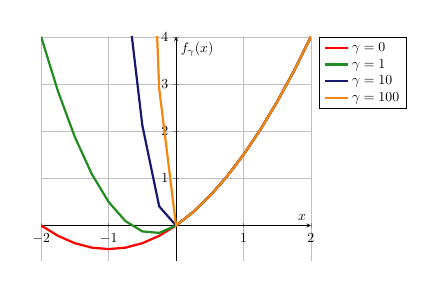
\begin{tikzpicture}[scale=0.5]
    \begin{axis}[
        axis lines=middle, % Draw axes through the origin
        xlabel=$x$,
        ylabel=$f_\gamma(x)$,
        xmin=-2, xmax=2, % Adjust x-range as needed
        ymin=-0.75, ymax=4, % Adjust y-range as needed
        grid=both, % Add a grid
        grid style={line width=.1pt, draw=gray!10}, % Style the grid lines
        major grid style={line width=.2pt,draw=gray!50}, % Style major grid lines
        xtick distance=1, % Tick marks every 1 unit on x-axis
        ytick distance=1, % Tick marks every 1 unit on y-axis
        % Add a legend
        legend pos=outer north east, % Position the legend
        legend cell align=left,
        no markers, % Don't put markers on the plots
    ]

    % Define the function with a placeholder for c
    % We use 'max(0,x)^2' for the (x)^2 part, and then multiply by c
    % PGFPlots works with degrees, so we need to be careful with functions that are not trigonometric.
    % max(0, x) is directly supported.


    \addplot[domain=-2:4, Red, ultra thick] {0.5*x^2 + 1*x + 0 * max(0,-x)^2};
    \addlegendentry{$\gamma=0$};
    % Plot for c = 0.5
    \addplot[domain=-2:4, ForestGreen, ultra thick] {0.5*x^2 + 1*x + 1 * max(0,-x)^2};
    \addlegendentry{$\gamma=1$};

    % Plot for c = 1
    \addplot[domain=-2:4, MidnightBlue, ultra thick] {0.5*x^2 + 1*x + 10.0 * max(0,-x)^2};
    \addlegendentry{$\gamma=10$};

    % Plot for c = 2
    \addplot[domain=-2:4, BurntOrange, ultra thick] {0.5*x^2 + 1*x + 50.0 * max(0,-x)^2};
    \addlegendentry{$\gamma=100$};

    \end{axis}
\end{tikzpicture}
%}
\caption{\scriptsize Plot of $f_\gamma(x) = \frac{1}{2} x^2 + x + \gamma\max\{0,-x\}^2$}
  \label{fig:tikz-example}
\end{figure}
\end{minipage}
  \end{frame}
  
  \begin{frame}\frametitle{A Workflow for Penalty Methods}
     \visible<1->{
 \begin{beamercolorbox}[rounded=true, shadow=true, wd=\textwidth]{block title}\centering
The $\gamma$-dependent subproblems are no longer constrained. This makes both the analysis and the numerical solution more familiar to techniques for PDEs.
 \end{beamercolorbox}}\hfill
 
 \visible<2->{
 \begin{beamercolorbox}[rounded=true, shadow=true, wd=\textwidth]{block body}
\visible<3->{Theory: 
\begin{itemize}
\item \visible<4->{Prove existence and uniqueness of $u_{\gamma}$ using the Direct Method.}
\item \visible<5->{Prove that $J_{\gamma} \to J + i_{K}$ in the sense of \alert{Mosco convergence} $\Rightarrow$ $u_{\gamma} \rightharpoonup u$.}
\item \visible<6->{Prove that $J_{\gamma}$ is G\^{a}teaux differentiable and derive optimality conditions:
\[
dJ_{\gamma}(u_{\gamma}) = 0 \Leftrightarrow -\Delta u - \underbrace{\gamma \max\{0,\varphi-u\}}_{=:\lambda_{\gamma}} = f.
\]}
\end{itemize}
}\vspace{-3ex}

%\visible<7->{Algorithms:
%\begin{itemize}
%\item A standard way to compute $u_{\gamma}$ is the \alert{Semismooth Newton Method}.
%\item In a nutshell: Given $u^k \in H^1_0(\Omega)$, compute $\delta^k \in H^1_0(\Omega)$ such that
%\[
%-\Delta \delta
%\]
%\end{itemize}
%}
 \end{beamercolorbox}}
  \end{frame}
  
    \begin{frame}\frametitle{A Workflow for Penalty Methods}
      \visible<1->{
 \begin{beamercolorbox}[rounded=true, shadow=true, wd=\textwidth]{block title}\centering
Both theory and experience has shown that developing algorithms in infinite dimensions (usually) leads to mesh independent numerical methods after discretization.
 \end{beamercolorbox}}\hfill   
    
 \begin{beamercolorbox}[rounded=true, shadow=true, wd=\textwidth]{block body}
\visible<2->{Algorithms:
\begin{itemize}
\item \visible<2->{A standard way to compute $u_{\gamma}$ is the \alert{Semismooth Newton Method}.}
\item \visible<3->{In a nutshell: Given $u^k \in H^1_0(\Omega)$, compute $\delta^k \in H^1_0(\Omega)$ such that
\[
-\Delta \delta^k + \gamma \chi_{\{\varphi - u^k > 0\}}\delta^k = \underbrace{\Delta u^k + \gamma \max\{0, \varphi - u^k\} + f}_{=:\tt{res_k}} 
\]\vspace{-2ex}}

\visible<4->{Set $u^{k+1} := u^k + \delta^k.$ Stop when $\|{\tt res_{k+1}}\|_{H^{-1}(\Omega)} \le {\tt tol_{rel}}\|{\tt res_{0}}\|_{H^{-1}(\Omega)} + {\tt tol_{abs}}$  }
\end{itemize}
}
 \end{beamercolorbox}
  \end{frame}

\begin{frame}\frametitle{Comments I}
 \begin{beamercolorbox}[rounded=true, shadow=true, wd=\textwidth]{block body}
\visible<1->{For each fixed $\gamma > 0$, this method provably converges \alert{very fast} (locally superlinearly).\medskip}
 
 \visible<2->{Analytical path-following methods for adaptive, automatic updates of $\gamma$ are available.\medskip} 
 
 \visible<3->{But $u_{\gamma}$ is \alert{never} feasible for \alert{finite} $\gamma$. This may cause \alert{conditioning issues} as $\gamma \uparrow +\infty$.}
  \end{beamercolorbox}
  
 \visible<4->{
  \begin{beamercolorbox}[rounded=true, shadow=true, wd=\textwidth]{block body}
  There are two challenges for discretization: 
  \[\aligned
  ( \chi_{\{\varphi - u^k > 0\}}\delta^k, w) &= \int_{\{\varphi - u^k > 0\}} \delta^k w \dd x\\
  ( \max\{0, \varphi - u^k\} ,w) &= \int_{\{\varphi - u^k > 0\}}(\varphi - u^k) w \dd x
  \endaligned
  \]
 \end{beamercolorbox}
 }
\end{frame}

\begin{frame}\frametitle{Comments II}
\begin{minipage}{0.3\textwidth}\centering
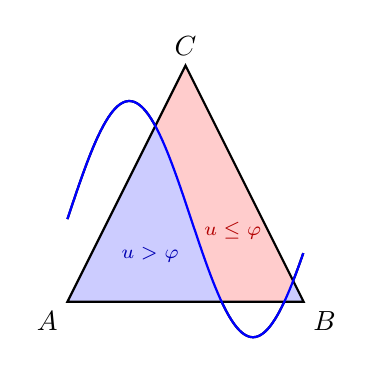
\begin{tikzpicture}[scale=3]
  % Define triangle vertices
  \coordinate (A) at (0,0);
%  \coordinate (B) at (1,0);
%  \coordinate (C) at (0.5,1);

  \coordinate (B) at (1,0);
  \coordinate (C) at (0.5,1);

  % Define curve
  \draw[name path=curve, thick, domain=0:1, samples=100, variable=\x] 
    plot ({\x}, {0.5*sin(6*\x r) + 0.35});

  % Triangle path
  \path[name path=AB] (A) -- (B);
  \path[name path=BC] (B) -- (C);
  \path[name path=CA] (C) -- (A);

  % Clip and fill region below curve inside triangle
  \begin{scope}
    \clip (A) -- (B) -- (C) -- cycle;
    \fill[blue!20] plot[domain=0:1, samples=100] 
      ({\x}, {0.5*sin(6*\x r) + 0.35}) -- (1,0) -- (0,0) -- cycle;
  \end{scope}

  % Clip and fill region above curve inside triangle
  \begin{scope}
    \clip (A) -- (B) -- (C) -- cycle;
    \fill[red!20] (0,0) -- (0.5,1) -- (1,0) -- 
      plot[domain=1:0, samples=100] 
      ({\x}, {0.5*sin(6*\x r) + 0.35}) -- cycle;
  \end{scope}

  % Draw triangle edges
  \draw[thick] (A) -- (B) -- (C) -- cycle;

  % Draw curve on top
  \draw[thick, blue] plot[domain=0:1, samples=100] 
    ({\x}, {0.5*sin(6*\x r) + 0.35});

  % Optional: label triangle vertices
  \node[below left] at (A) {$A$};
  \node[below right] at (B) {$B$};
  \node[above] at (C) {$C$};
  
 
   % Label in blue region (below the curve)
  \node[blue!70!black] at (0.35,0.2) {\scriptsize $u > \varphi$};

  % Label in red region (above the curve)
  \node[red!70!black] at (0.7,0.3) {\scriptsize $u \le \varphi$};
\end{tikzpicture}
\end{minipage}\hfill
\begin{minipage}{0.68\textwidth}
  \begin{beamercolorbox}[rounded=true, shadow=true, wd=\textwidth]{block body}
  To be computationally efficient, we need to make a choice:\medskip
  
For a cell $T$, we are given
\begin{enumerate}
\item Quadrature points $x_1,\dots,x_p$
\item Weights $w_1,\dots,w_p$
\item $N_{T} = \{1,\dots,p\}$ 
\end{enumerate}\visible<2->{
\alert{If $\varphi(x_i) - u^k(x_i) \le 0$, then $N_{T} := N_{T} \setminus \{i\}$}.}\visible<3->{
Then we use
  \[\aligned
  ( \chi_{\{\varphi - u^k > 0\}}\delta^k, v) &\approx \sum_{i \in N_{T}}w_i \delta^k(x_i) v(x_i)\\
  ( \max\{0, \varphi - u^k\} ,v) &\approx \sum_{i \in N_{T}}w_i(\varphi(x_i) - u^k(x_i)) v(x_i).
  \endaligned
  \]\vspace{-1ex}}
 \end{beamercolorbox}
\end{minipage}
\end{frame}

\begin{frame}\frametitle{Augmented Lagrangian Method}
      \visible<1->{
 \begin{beamercolorbox}[rounded=true, shadow=true, wd=\textwidth]{block title}\centering
The conditioning issues and lack of guarantees for feasibilty are a major downside of penalty methods.
 \end{beamercolorbox}}\hfill   
 
       \visible<2->{
 \begin{beamercolorbox}[rounded=true, shadow=true, wd=\textwidth]{block body}\centering
Finite-dimensional nonlinear optimization offers a (sort of) remedy to this problem in the form of the \alert{Augmented Lagrangian Method}.
 \end{beamercolorbox}}\hfill    
 
       \visible<3->{
 \begin{beamercolorbox}[rounded=true, shadow=true, wd=\textwidth]{block body}\centering
In \alert{finite dimensions} we do not require the penalty parameter to pass to infinity for AL.
 \end{beamercolorbox}}
\end{frame}

  \begin{frame}\frametitle{Augmented Lagrangian Method}
  \begin{minipage}{0.68\linewidth}
\begin{beamercolorbox}[rounded=true, shadow=true, wd=\textwidth]{block body}
 Given $\gamma > 0$, and a Lagrange multiplier $\lambda$, we define the \alert{Lagrangian} and \alert{Augmented Lagrangian}, resp.:
 \begin{equation*}\aligned
  	L(v,\lambda)
 	&=
	\frac{1}{2}\| \nabla v \|^2 - (f,v) - \langle \lambda, v-\varphi\rangle\\
 	L(v,\lambda,\gamma)
 	&=
 	\frac{1}{2}\| \nabla v \|^2 - (f,v) -  \| \lambda\|^2\\
	&\hspace{8ex}+
	\frac{1}{2\gamma}\|(\lambda + \gamma (\varphi - u))_+\|^2
 	\endaligned
 \end{equation*}
\end{beamercolorbox}
\end{minipage}\hfill
\begin{minipage}{0.3\linewidth}
 \begin{figure}
% \resizebox{0.3\textwidth}{0.25\textwidth}{%
  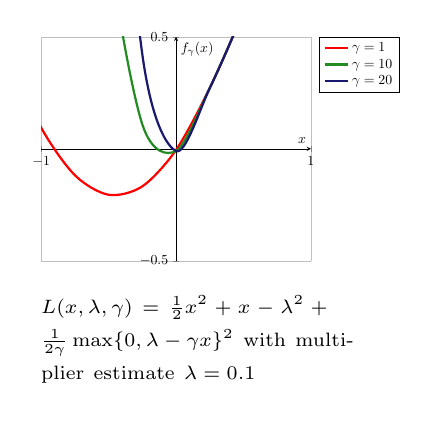
\begin{tikzpicture}[scale=0.5]
    \begin{axis}[
        axis lines=middle, % Draw axes through the origin
        xlabel=$x$,
        ylabel=$f_\gamma(x)$,
        xmin=-1, xmax=1, % Adjust x-range as needed
        ymin=-0.5, ymax=.5, % Adjust y-range as needed
        grid=both, % Add a grid
        grid style={line width=.1pt, draw=gray!10}, % Style the grid lines
        major grid style={line width=.2pt,draw=gray!50}, % Style major grid lines
        xtick distance=1, % Tick marks every 1 unit on x-axis
        ytick distance=.5, % Tick marks every 1 unit on y-axis
        % Add a legend
        legend pos=outer north east, % Position the legend
        legend cell align=left,
        no markers, % Don't put markers on the plots
    ]

    % Define the function with a placeholder for c
    % We use 'max(0,x)^2' for the (x)^2 part, and then multiply by c
    % PGFPlots works with degrees, so we need to be careful with functions that are not trigonometric.
    % max(0, x) is directly supported.


    \addplot[domain=-2:4, Red, ultra thick, smooth] {0.5*x^2 + 1*x  - 0.1^2 + 1 * max(0,0.1-x)^2 / 2};
    \addlegendentry{$\gamma=1$};
    % Plot for c = 0.5
    \addplot[domain=-2:4, ForestGreen, ultra thick,smooth] {0.5*x^2 + 1*x  - 0.1^2 + max(0,0.1-10*x)^2 / (2*10)};
    \addlegendentry{$\gamma=10$};

    % Plot for c = 1
    \addplot[domain=-2:4, MidnightBlue, ultra thick, smooth] {0.5*x^2 + 1*x - 0.1^2+  max(0,0.1-20*x)^2 / (2*20)};
    \addlegendentry{$\gamma=20$};

    % Plot for c = 2
%    \addplot[domain=-2:4, BurntOrange, ultra thick] {0.5*x^2 + 1*x  - x + 50.0 * max(0,-x)^2 * 0.5};
%    \addlegendentry{$\gamma=50$};
	
    \end{axis} \node[text width=4cm, align=left] at (4,-2) {\scriptsize $L(x,\lambda,\gamma) =\frac{1}{2} x^2 + x -\lambda^2 + \frac{1}{2\gamma}\max\{0,\lambda-\gamma x\}^2$ with multiplier estimate $\lambda = 0.1$};
\end{tikzpicture}
%}
%\caption{\scriptsize Plot of $L(x,\lambda,\gamma) =\frac{1}{2} x^2 + x -\lambda + \gamma\max\{0,-x\}^2$ with $\lambda = 0.5$}
  \label{fig:tikz-example}
\end{figure}
\end{minipage}
      \visible<1->{
 \begin{beamercolorbox}[rounded=true, shadow=true, wd=\textwidth]{block title}\centering
In light of the theory of Lagrange multipliers for the obstacle problem ($\lambda \in H^{-1}(\Omega) \cap M(\Omega)$), there is a clear discrepancy. Here, we need $\lambda \in L^2(\Omega)$.
 \end{beamercolorbox}}\hfill   
  \end{frame}
  
  \begin{frame}\frametitle{AL Workflow}
  \visible<1->{
   \begin{beamercolorbox}[rounded=true, shadow=true, wd=\textwidth]{block body}
\visible<1->{The theory for the subproblems  mirrors that of penalty methods (if $\lambda$ is regular).\medskip

\visible<2->{The optimality conditions for minimizing $L(u,\lambda,\gamma)$ are
\[
-\Delta u - \max\{0,\lambda + \gamma(\varphi - u)\} = f
\]
We can therefore compute $u_{\gamma}$ using a \alert{Semismooth Newton Method}.\medskip}

\visible<3->{We take $\gamma := \tau\gamma$ ($\tau > 1$) and \alert{update} the \alert{multipliers} $\lambda_{\gamma}$ using the formula 
\[
\lambda_{\gamma} := \lambda + \max\{0,\lambda + \gamma(\varphi - u_{\gamma})\}.
\]
}\vspace{-3ex}
}
\end{beamercolorbox}}   
  
        \visible<4->{
 \begin{beamercolorbox}[rounded=true, shadow=true, wd=\textwidth]{block title}
Ito \& Kunisch (1990) provides convergence theory for an AL method in Hilbert space that applies to the obstacle problem and a problem with gradient constraints.  \visible<3->{The theory requires more regularity of the obstacle, $\lambda \in L^2(\Omega)$, and $\gamma \to +\infty$.} \end{beamercolorbox}}\hfill   
  \end{frame}

\begin{frame}\frametitle{Interior Point Methods}
        \visible<1->{
 \begin{beamercolorbox}[rounded=true, shadow=true, wd=\textwidth]{block title}\centering
The previously sketched methods approximate the feasible set $K$ from ``the outside''. Classical interior point methods offer an alternative viewpoint.
\end{beamercolorbox}}   \vspace{3ex}
\visible<2->{
  \begin{minipage}{0.67\linewidth}
\begin{beamercolorbox}[rounded=true, shadow=true, wd=\textwidth]{block body}
 Given $\mu > 0$, use a \alert{logarithmic barrier function} and consider
 \begin{equation*}
 	J_{\mu}(v)
 	=
 	\frac{1}{2}
 	\int_\Omega |\nabla v|^2 \dd x
 	-
 	\int_\Omega f v\dd x
	-
	\mu \int_{\Omega} \ln(u-\varphi) \dd x
 	\,.
 \end{equation*}
\end{beamercolorbox}
\end{minipage}\hfill
\begin{minipage}{0.3\linewidth}
 \begin{figure}
 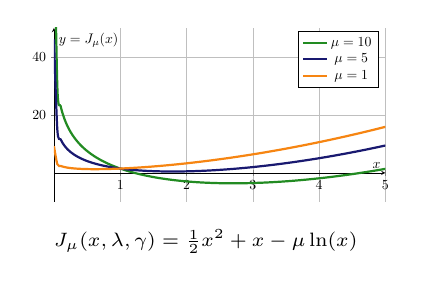
\begin{tikzpicture}[scale=0.5]
  \begin{axis}[
    domain=0.0001:5,
    samples=100,
    axis lines=middle,
    xlabel=$x$,
    ylabel={$y = J_\mu(x)$},
    ymin=-10, ymax=50,
    grid=both,
    width=10cm,
    height=6cm,
  ]
    \addplot[ForestGreen, ultra thick,smooth] {0.5*x^2 + 1*x - 10*ln(x)};
    \addlegendentry{$\mu=10$}
    
    \addplot[MidnightBlue, ultra thick, smooth] {0.5*x^2 + 1*x - 5*ln(x)};
    \addlegendentry{$\mu=5$}
    
    \addplot[ BurntOrange, ultra thick, smooth] {0.5*x^2 + 1*x - 1*ln(x)};
    \addlegendentry{$\mu=1$}
  \end{axis}
  \node[text width=4cm, align=left] at (4,-1) {\scriptsize $J_{\mu}(x,\lambda,\gamma) =\frac{1}{2} x^2 + x -\mu\ln(x)$};
\end{tikzpicture}
  \label{fig:tikz-example}
\end{figure}
\end{minipage}}
\end{frame}

\begin{frame}\frametitle{IP Workflow}
  \visible<1->{
   \begin{beamercolorbox}[rounded=true, shadow=true, wd=\textwidth]{block body}
\visible<1->{The theory for the subproblems is more complicated than for penalty and AL.\medskip

}
\visible<2->{Logarithmic penalties are \alert{not differentiable} in the usual functions spaces.\medskip

}
\visible<3->{If there are reals $\epsilon(\mu) > 0$ and $M(\mu) > 0$ such that solution $u_{\mu} \in [\varphi + \epsilon(\mu), M(\mu)]$, then 
\begin{multline*}
\int_{\Omega} \ln(u + \eta \delta - \varphi) - \ln(u-\varphi) - \eta\frac{\delta}{u - \varphi} \dd x =
-\eta^2 \underbrace{\left(\int_{\Omega}\frac{\delta}{u - \varphi}\int_{0}^{1} \frac{1}{u - \varphi +  \tau \eta \delta} \dd \tau\dd x.\right)}_{=: A(u,\delta,\eta)}
\end{multline*}\vspace{-2ex}

is valid provided $\eta > 0$ is sufficiently small and \alert{$\delta \in H^1(\Omega) \cap L^{\infty}(\Omega)$}.\medskip

}
\visible<4->{Once we show $A(u,\delta,\eta)$ is bounded as $\eta \downarrow 0$, we can derive the \alert{optimality condition}:
\[
J_{\mu}(u_{\mu}) = 0 \Longleftrightarrow -\Delta u_{\mu} - \frac{\mu}{u_{\mu} - \varphi} = f
\]
}\vspace{-3ex}
\end{beamercolorbox}}   
  
%        \visible<4->{
% \begin{beamercolorbox}[rounded=true, shadow=true, wd=\textwidth]{block title}
%Ito \& Kunisch (1990) provides convergence theory for an AL method in Hilbert space that applies to the obstacle problem and a problem with gradient constraints.  \visible<3->{The theory requires more regularity of the obstacle, $\lambda \in L^2(\Omega)$, and $\gamma \to +\infty$.} \end{beamercolorbox}}\hfill   

\end{frame}

\begin{frame}\frametitle{Comments I}
  \visible<1->{
   \begin{beamercolorbox}[rounded=true, shadow=true, wd=\textwidth]{block body}
\visible<1->{The optimality conditions yields a \alert{singular semilinear elliptic PDE}:
\[
-\Delta u_{\mu} - \frac{\mu}{u_{\mu} - \varphi} = f
\]
This is unfortunate, especially if the Lebesgue measure of $\mathcal{A} := \left\{u = \varphi \right\}$ is positive.\medskip 
}

\visible<2->{
Introducing a slack $\lambda_{\mu} := \frac{\mu}{u_{\mu} - \varphi}$ we can write down a \alert{primal dual} formulation:
\[\aligned
-\Delta u_{\mu} - \lambda_{\mu} &= f\\
(u_{\mu}-\varphi) \lambda_{\mu} &= \mu
\endaligned
\]
This system can be solved with \alert{Newton's method} for each $\mu$.}
\end{beamercolorbox}}   
  
%        \visible<4->{
% \begin{beamercolorbox}[rounded=true, shadow=true, wd=\textwidth]{block title}
%Ito \& Kunisch (1990) provides convergence theory for an AL method in Hilbert space that applies to the obstacle problem and a problem with gradient constraints.  \visible<3->{The theory requires more regularity of the obstacle, $\lambda \in L^2(\Omega)$, and $\gamma \to +\infty$.} \end{beamercolorbox}}\hfill   

\end{frame}

\begin{frame}\frametitle{Comments II}
  \visible<1->{
   \begin{beamercolorbox}[rounded=true, shadow=true, wd=\textwidth]{block body}
\visible<1->{Find strictly feasible $(u_{\mu},\lambda_{\mu})$ satisfying
\[\aligned
-\Delta u_{\mu} - \lambda_{\mu} &= f\\
(u_{\mu}-\varphi) \lambda_{\mu} &= \mu
\endaligned
\]}\visible<2->{We need to ensure $u_{\mu} > \varphi$ and $\lambda_{\mu} > 0$ to be faithful to interior point.\medskip

This does not guarantee feasibility and will require an intelligent strategy for updating $\mu$ and a special line search at each step to guarantee primal and dual feasibility.
}
\end{beamercolorbox}}   
  
        \visible<3->{
 \begin{beamercolorbox}[rounded=true, shadow=true, wd=\textwidth]{block title}\centering
Despite its theoretical promises, IP falls short of our ideal solver. \textbf{Is there a better idea?}
\end{beamercolorbox}}\hfill   

\end{frame}

%\section{The Bregman Proximal Point Method}
 \begin{frame}\frametitle{A better idea?}
%    \begin{enumerate}
%    	\item Martinet, Rockafellar
%	\item Bregman, Nemirovskij Yudin
%	\item Convergence statements
%    \end{enumerate}
    
\begin{beamercolorbox}[rounded=true, shadow=true, wd=\textwidth]{block body}
Each method we discussed above has a useful feature
\begin{enumerate}
\item \visible<2->{\textbf{Penalty methods} can be applied to any type of inequality constraint.}
\item \visible<3->{\textbf{Augmented Lagrangian methods} work like penalty methods but provide a dual-adapted penalty function at each step.\\
There pre-asymptotic feasibility guarantees in finite dimensions.}
\item \visible<4->{\textbf{Interior point methods} work with strictly feasible points.}
\end{enumerate}
\end{beamercolorbox}\hfill

\visible<5->{
 \begin{beamercolorbox}[rounded=true, shadow=true, wd=\textwidth]{block title}\centering
The \textbf{Bregman proximal point method} offers an alternative for the obstacle problem.
\end{beamercolorbox}
}\hfill

\visible<6->{
 \begin{beamercolorbox}[rounded=true, shadow=true, wd=\textwidth]{block body}\centering
In \alert{Part III} we will return to this perspective and derive a whole new class of methods for large classes of inequality constrained problems and beyond.
\end{beamercolorbox}
}
 \end{frame}

\section{Derivation of the Latent Variable Proximal Point Method}
 \begin{frame}\frametitle{Frame Title}
        \begin{enumerate}
    	\item Formal application to the obstacle problem
	\item Failure of the primal version
	\item Invention of the latent variable
	\item Discretization approaches
    \end{enumerate}
 \end{frame}
 
 \begin{frame}\frametitle{A Brief History of Proximal Point}
        \visible<1->{
 \begin{beamercolorbox}[rounded=true, shadow=true, wd=\textwidth]{block body}
\visible<1->{Lions \& Stampacchia (1967): The non-symmetric part of the proof  in Part I is deeply linked to \alert{Proximal Gradient Methods}.\medskip}

\visible<2->{B. Martinet (1970): Invention of the \alert{Proximal Point Method} for variational inequalities:
\begin{center}
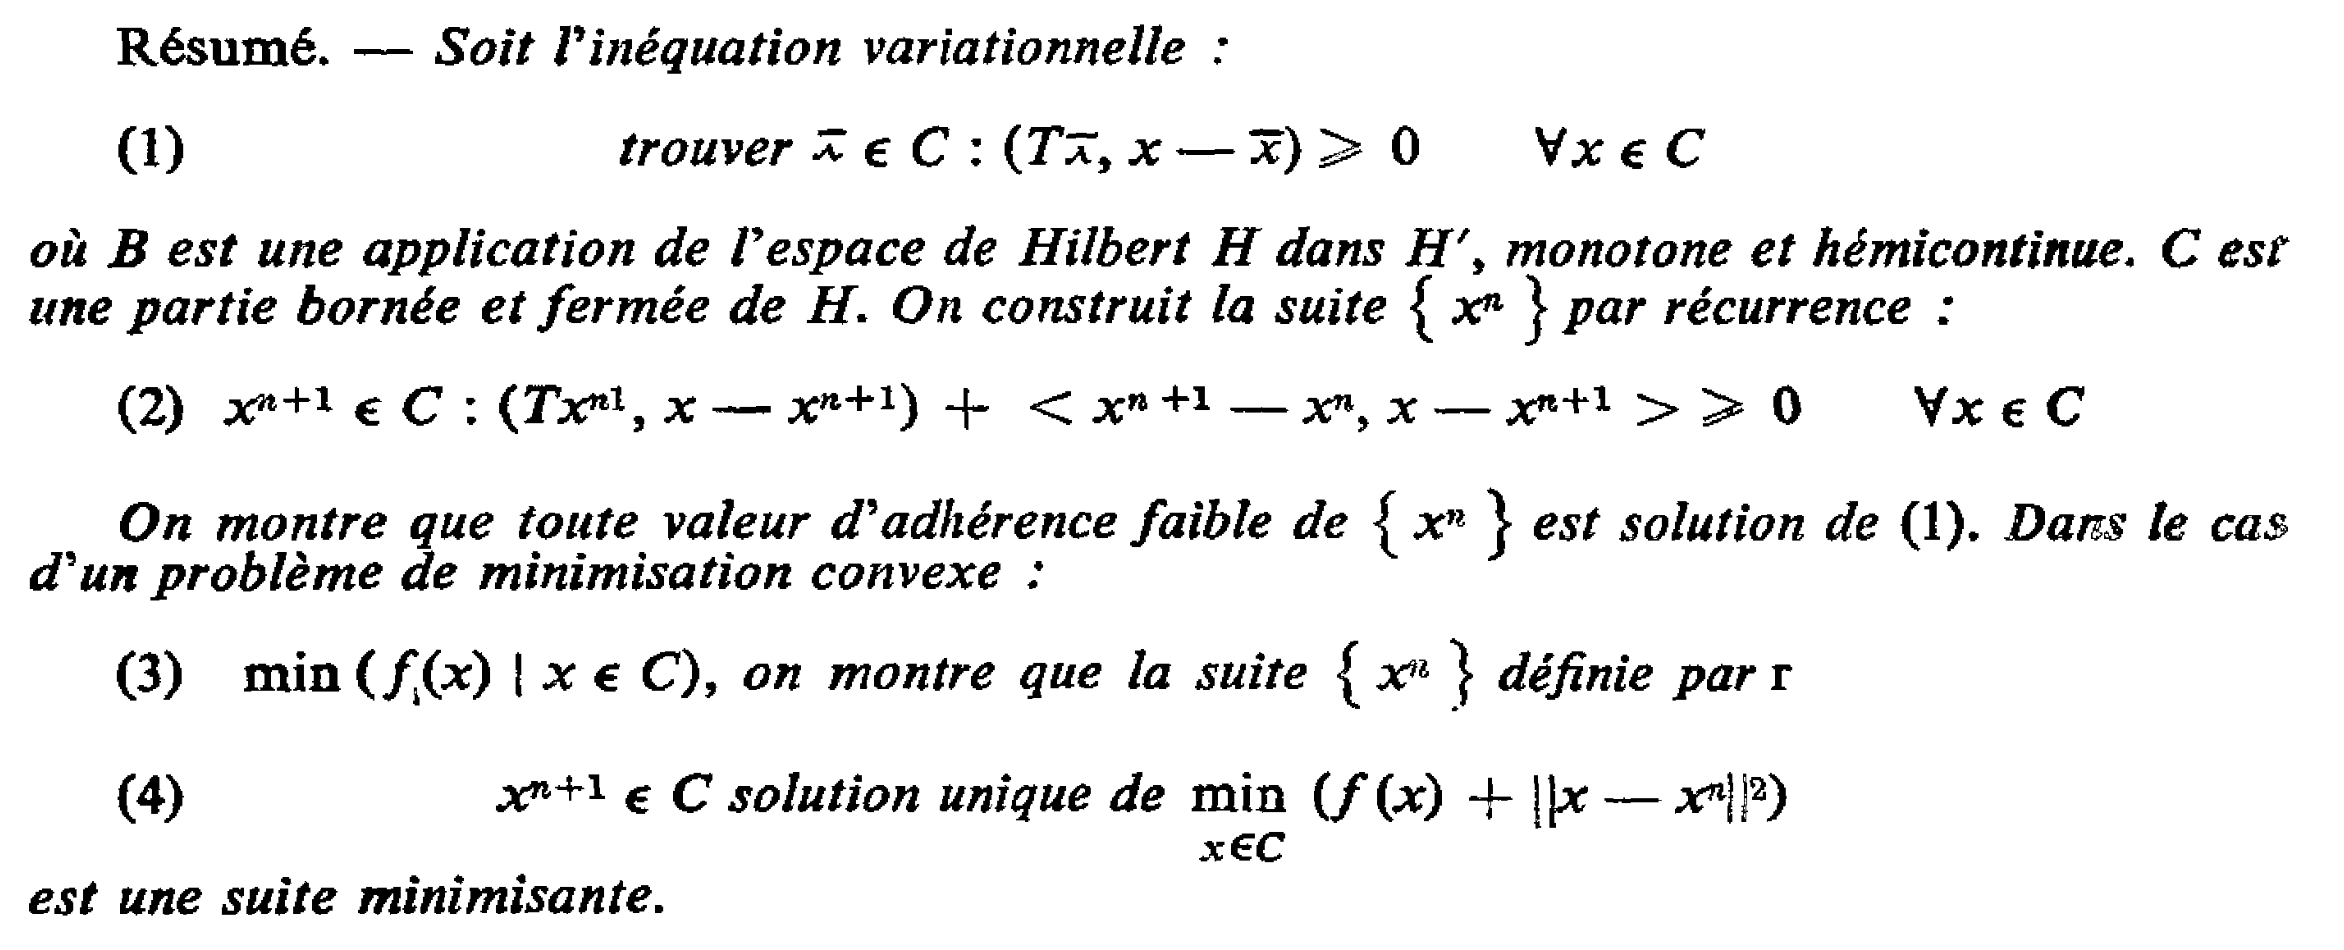
\includegraphics[height=1.25in,keepaspectratio]{figures/bmartinet_1970_summary.png}
\end{center}}
\visible<3->{
Rockafellar (1976), G\"uler (1991): Generalizations and main convergence statements. }
\end{beamercolorbox}}   \vspace{3ex}
\end{frame}
 

\begin{frame}\frametitle{Application to Obstacle Problem}
 \begin{beamercolorbox}[rounded=true, shadow=true, wd=\textwidth]{block body}
 	Applying this idea to the Obstacle Problem leads to the variational inequality:
	\begin{equation*}
%	\label{eq:L2ProxVI}
		\int_\Omega
		\nabla( (1+\alpha)u - u^{k}) \cdot \nabla w
		\dd x
		+
		\int_\Omega (u-u^{k}-\alpha f) w  \dd x
		\geq
		0
		~\fa w \in K-u,\quad \alpha > 0
	\end{equation*}
	But this is \alert{as difficult to solve as} the original VI!
 \end{beamercolorbox}
 \visible<2->{
 \begin{beamercolorbox}[rounded=true, shadow=true, wd=\textwidth]{block title}\centering
 The idea to use a regularization that includes information from the previous iterate $u^{k}$ is similar to AL (where we used $\lambda^{k}$).
 \end{beamercolorbox}}
 \visible<3->{
  \begin{beamercolorbox}[rounded=true, shadow=true, wd=\textwidth]{block body}
But the regularization
\[
u \mapsto \frac{1}{2\alpha} \| u - u^{k} \|^2_{H^1}
\]
is essentially \alert{useless}. There are, however, bivariate functions that behave similarly.
 \end{beamercolorbox}}
\end{frame}

 \begin{frame}\frametitle{Alternative Regularizations}
 \visible<1->{
  \begin{minipage}{0.67\linewidth}
\begin{beamercolorbox}[rounded=true, shadow=true, wd=\textwidth]{block body}
L.M. Bregman (1967): \visible<2->{Given a \alert{distance-generating functions} $R$,
the associated \alert{Bregman distance} measures the linearization error of $R$:
\begin{equation*}
%\label{eq:BregmanDivergence}
D_R(a, b) := R(a) - R(b) - \nabla R(b) \cdot (a-b),
\end{equation*}
for all $a \in \mathop{\text{dom}} R,~b \in \mathop{\text{int}} \mathop{\text{dom}} R$.}
\end{beamercolorbox}
\end{minipage}\hfill
\begin{minipage}{0.3\linewidth}
 \begin{figure}
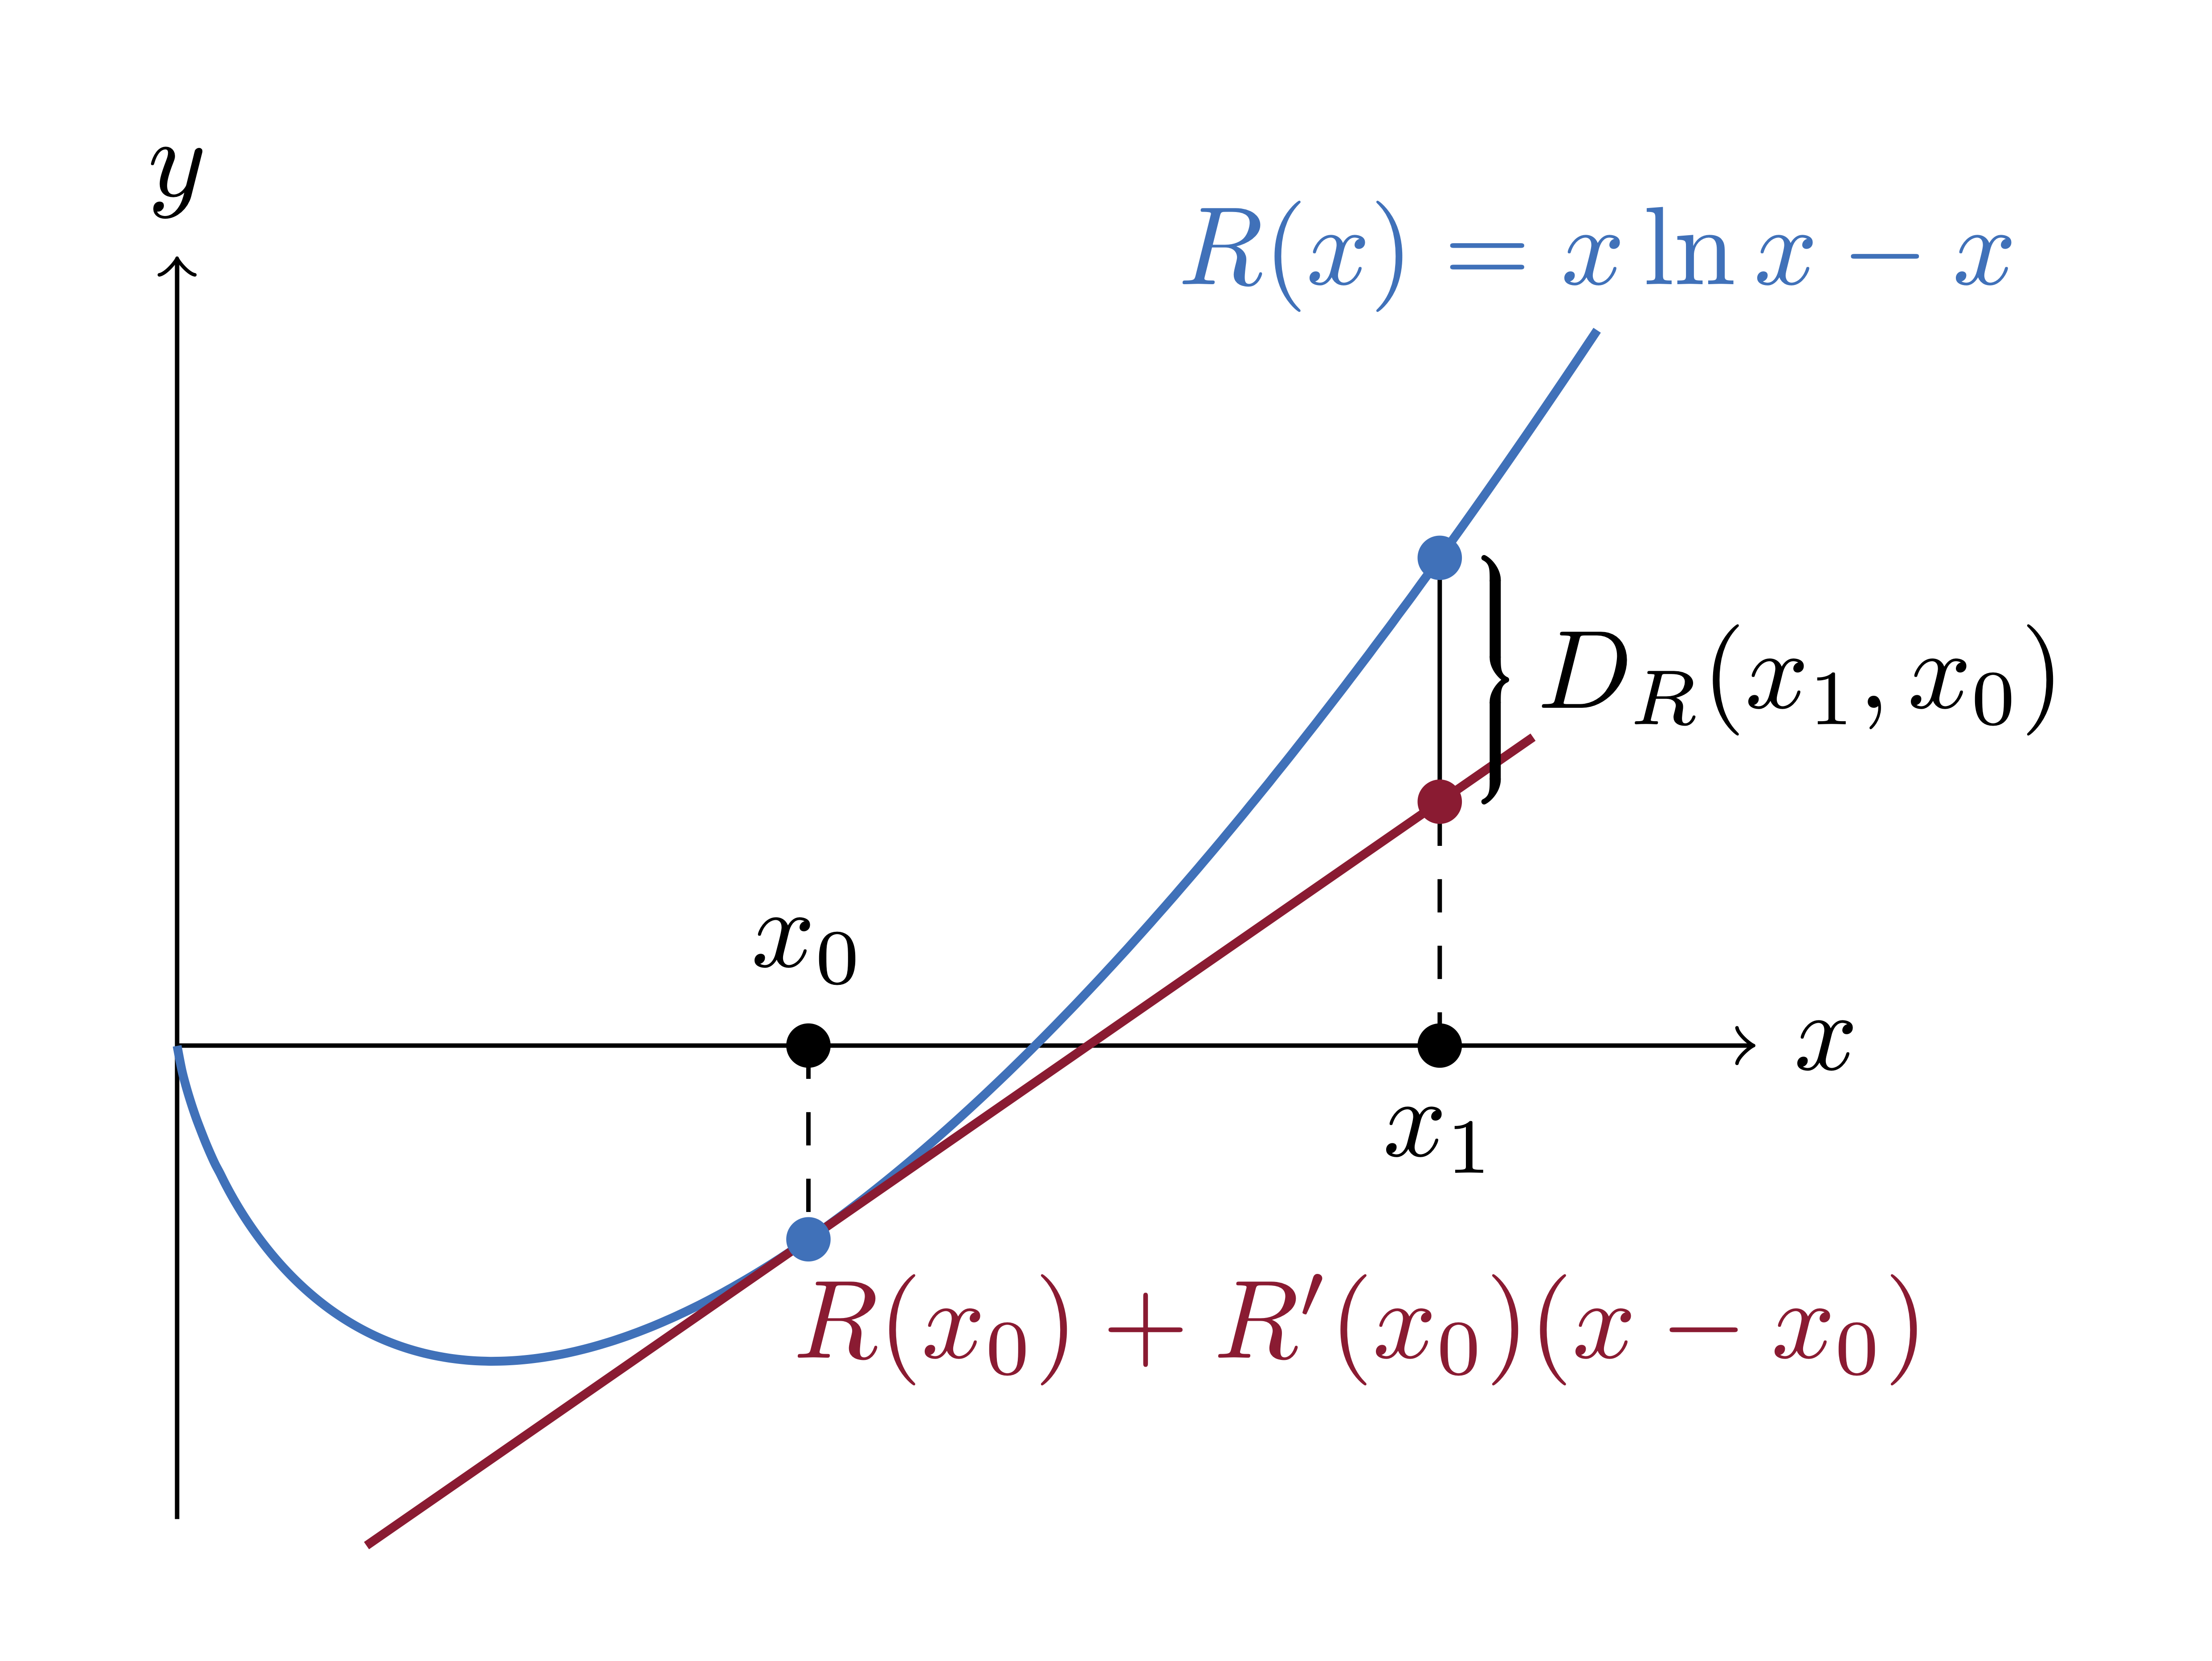
\includegraphics[height=1.25in,keepaspectratio]{figures/Bregman.png}
\end{figure}
\end{minipage}}

\visible<3->{
\begin{beamercolorbox}[rounded=true, shadow=true, wd=\textwidth]{block title}
Y. Censor \& S.A. Zenios (1992): Invention of the \textbf{Bregman Proximal Point Method}: Generate a sequence $\{u^k\}$\vspace{-2ex}
\[
u^{k+1} \in \mathrm{argmin}_{u \in V} \left\{J(u) + \frac{1}{\alpha^{k}} D(u,u^{k}) \right\}\quad \text{for}\quad \{\alpha^k\},\; \alpha^k > 0.
\]
G. Chen \& M. Teboulle (1993): Convergence proof based on G\"uler (1991).
\end{beamercolorbox}}
\end{frame}
 
  \begin{frame}\frametitle{Shannon Entropy \& Kullback-Leibler}
 \visible<1->{
  \begin{minipage}{0.67\linewidth}
\begin{beamercolorbox}[rounded=true, shadow=true, wd=\textwidth]{block body}
\visible<1->{The \alert{Shannon entropy} (C. Shannon (1948)) $R: \mathbb R_+ \to \mathbb R$:
\begin{equation*}
%\label{eq:GeneralizedShannonEntropy}
R(a) = a  \ln a  - a, %\text{ with } \nabla R^*(a^\ast) = \phi_1 + \exp{a^\ast},
\end{equation*}
yields
\[\aligned
D_{R}(a,b) 
&= a \ln a - a - (b \ln b - b + (\ln b + 1 - 1)(a-b))\\
&= a \ln \frac{a}{b} - (a- b)
\endaligned
\]
}
for all $a \in \mathop{\text{dom}} R = \mathbb R_+,~b \in \mathop{\text{int}} \mathop{\text{dom}} R = \mathbb R_{++}$.
\end{beamercolorbox}}
\end{minipage}\hfill
\begin{minipage}{0.3\linewidth}
 \begin{figure}
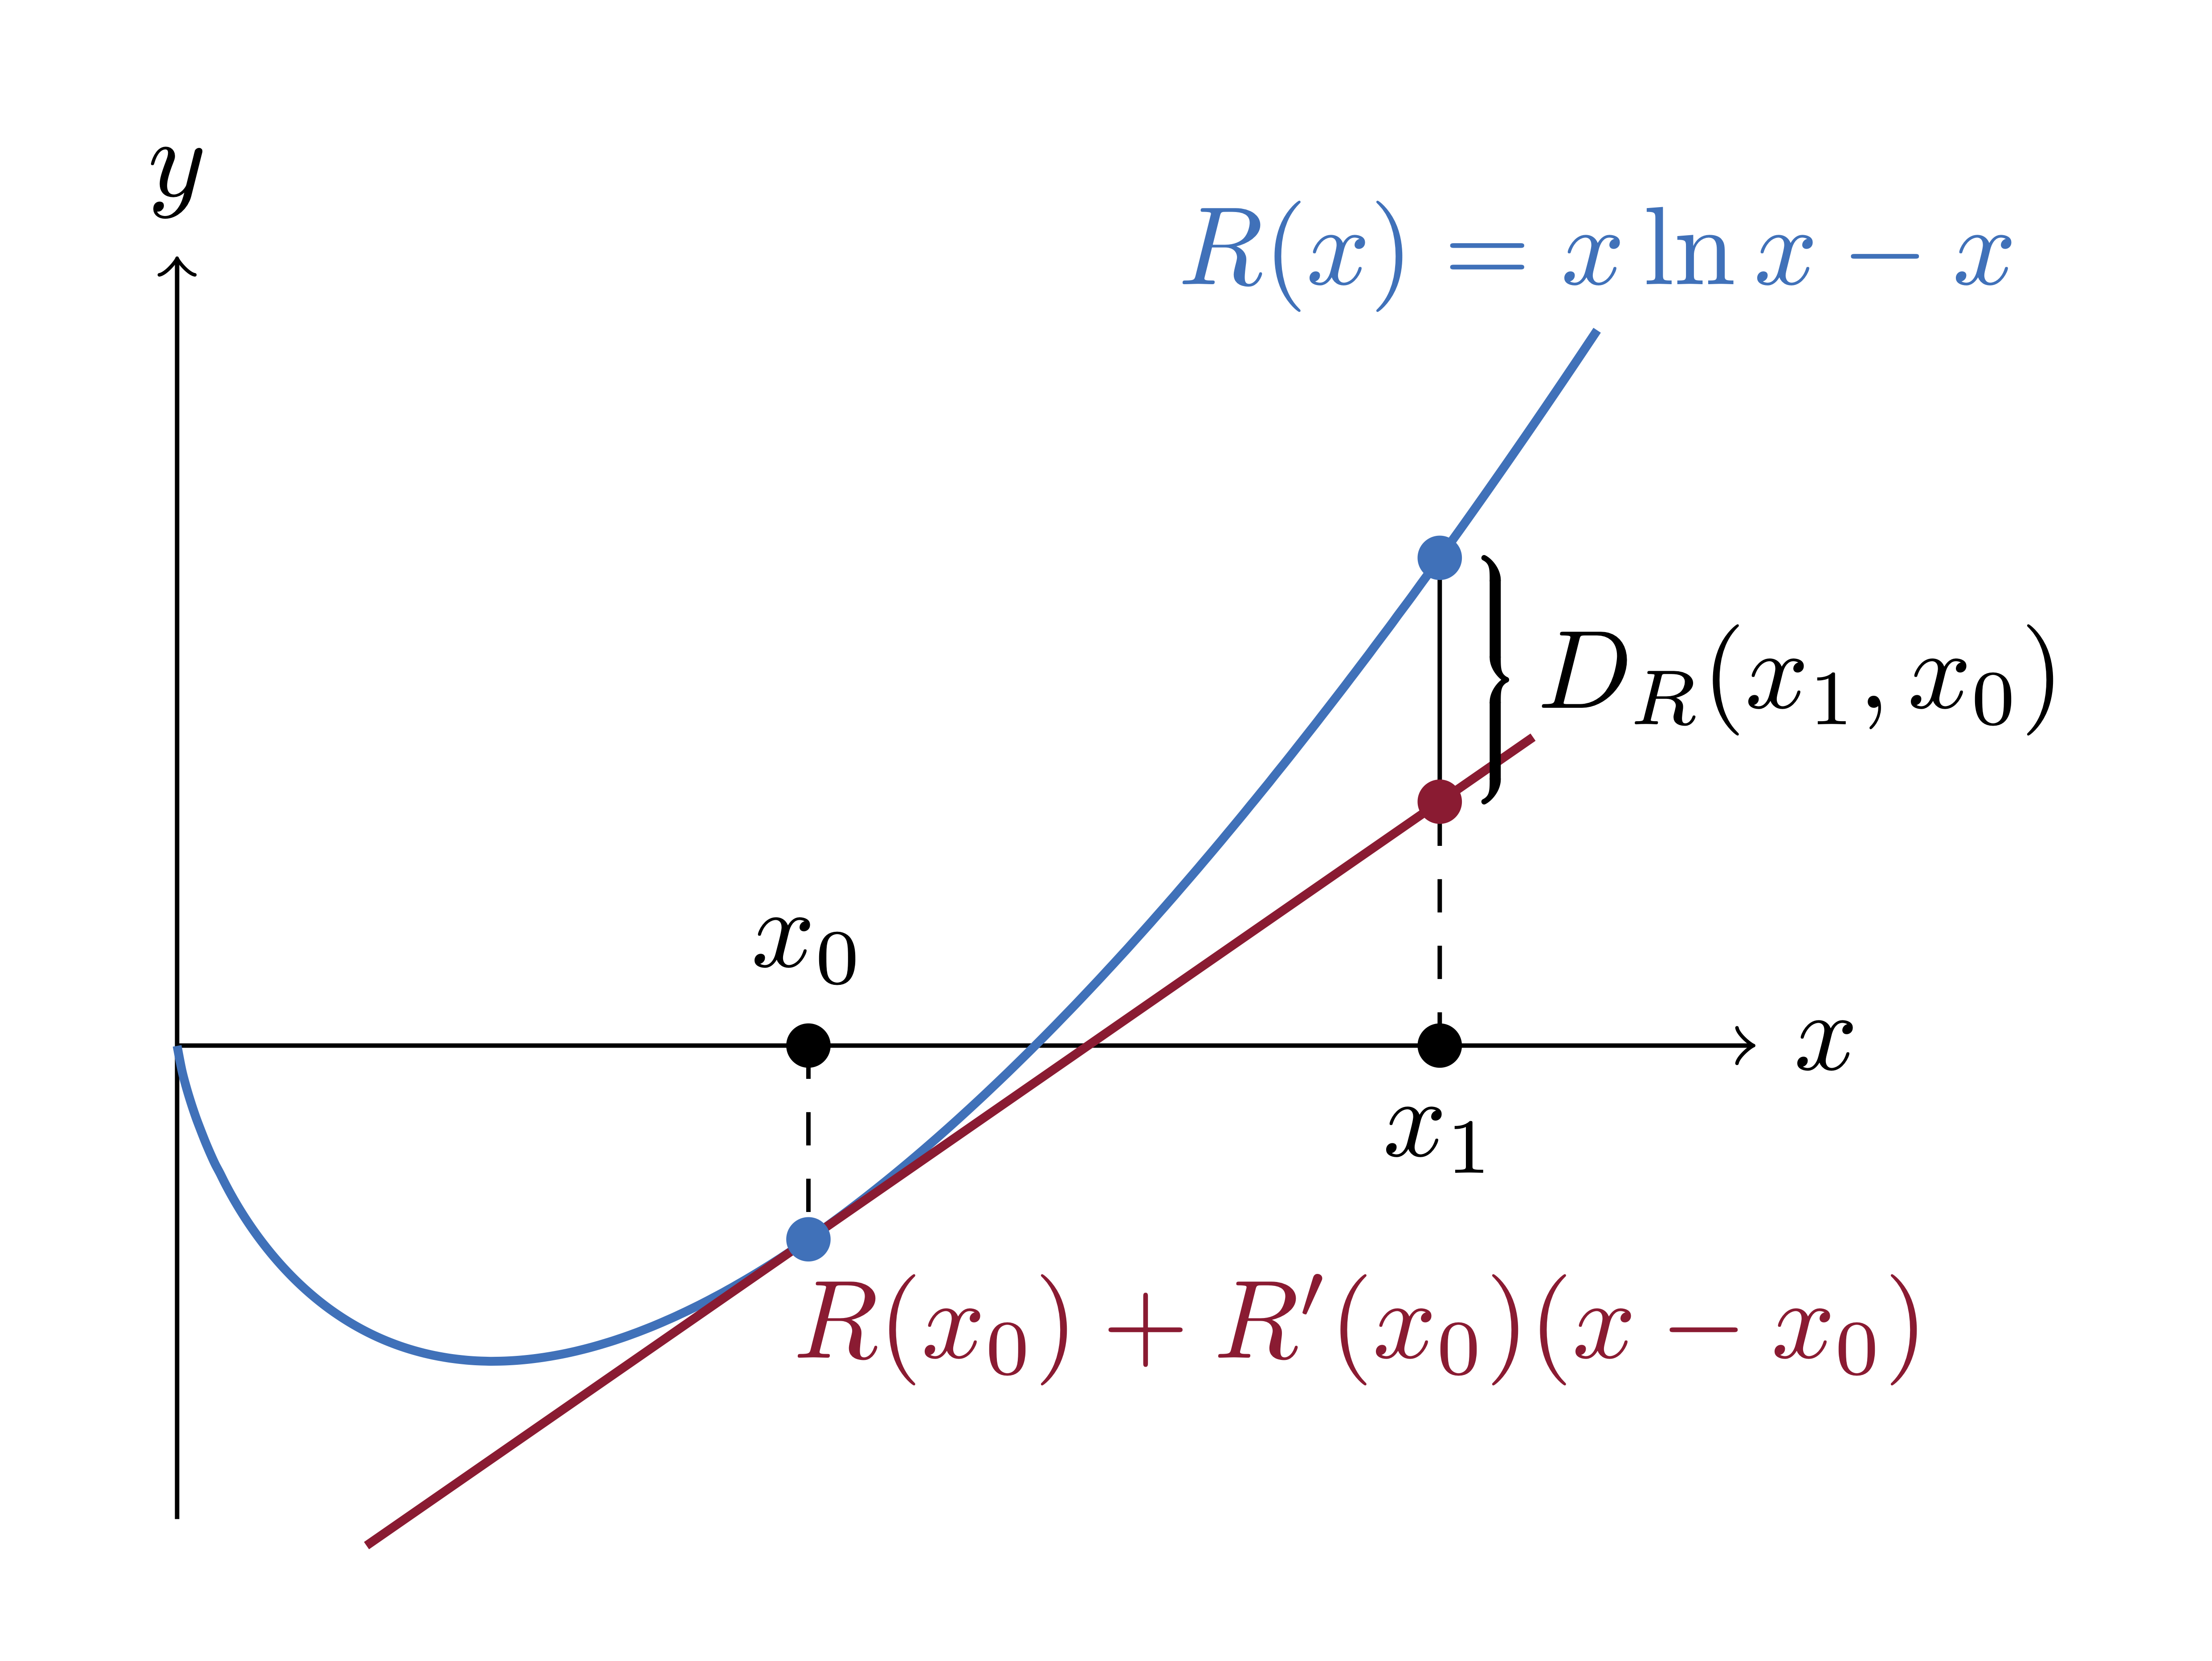
\includegraphics[height=1.25in,keepaspectratio]{figures/Bregman.png}
\end{figure}
\end{minipage}

\visible<2->{
\begin{beamercolorbox}[rounded=true, shadow=true, wd=\textwidth]{block body}
In other words, the Bregman divergence associated with the Shannon entropy is the well-known \alert{Kullback-Leibler divergence} (Kullback \& Leibler (1951)).
\end{beamercolorbox}}
 \end{frame}
 
   \begin{frame}\frametitle{Return to the Obstacle Problem}
  \begin{minipage}{0.68\linewidth}
\begin{beamercolorbox}[rounded=true, shadow=true, wd=\textwidth]{block body}
 Given $\alpha > 0$, and a previous iterate $v > \varphi$, we consider:
 \begin{equation*}\aligned
 	L(u,v,\alpha)
 	&=
 	\frac{1}{2}\| \nabla u \|^2 - (f,u)\\
	&\hspace{8ex}+
	\frac{1}{\alpha}\int_{\Omega} (u - \varphi) \ln \left(\frac{u - \varphi}{v - \varphi}\right) - (u - v)\dd x
 	\endaligned
 \end{equation*}
 Set $L(u,v,\alpha) = +\infty$ if $u < \varphi$ on a set of positive measure.
\end{beamercolorbox}
\end{minipage}\hfill
\begin{minipage}{0.3\linewidth}
 \begin{figure}
% \resizebox{0.3\textwidth}{0.25\textwidth}{%
  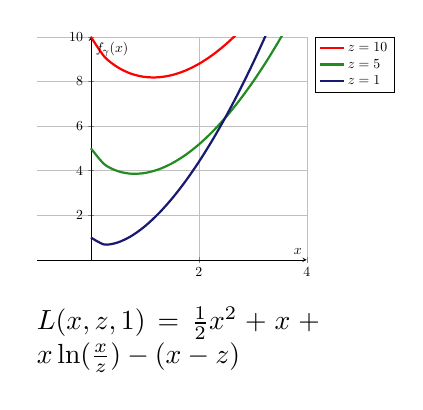
\begin{tikzpicture}[scale=0.5]
    \begin{axis}[
        axis lines=middle, % Draw axes through the origin
        xlabel=$x$,
        ylabel=$f_\gamma(x)$,
        xmin=-1, xmax=4, % Adjust x-range as needed
        ymin=-0.05, ymax=10, % Adjust y-range as needed
        grid=both, % Add a grid
        grid style={line width=.1pt, draw=gray!10}, % Style the grid lines
        major grid style={line width=.2pt,draw=gray!50}, % Style major grid lines
        xtick distance=2, % Tick marks every 1 unit on x-axis
        ytick distance=2, % Tick marks every 1 unit on y-axis
        % Add a legend
        legend pos=outer north east, % Position the legend
        legend cell align=left,
        no markers, % Don't put markers on the plots
    ]

    % Define the function with a placeholder for c
    % We use 'max(0,x)^2' for the (x)^2 part, and then multiply by c
    % PGFPlots works with degrees, so we need to be careful with functions that are not trigonometric.
    % max(0, x) is directly supported.


    \addplot[domain=-2:4, Red, ultra thick, smooth] {0.5*x^2 + 1*x  + (x * ln(x/10) - (x-10))/ 1};
    \addlegendentry{$z=10$};
    % Plot for c = 0.5
    \addplot[domain=-2:4, ForestGreen, ultra thick,smooth] {0.5*x^2 + 1*x   + (x * ln(x/5) - (x-5))/ (1)};
    \addlegendentry{$z=5$};

    % Plot for c = 1
    \addplot[domain=-2:4, MidnightBlue, ultra thick, smooth] {0.5*x^2 + 1*x +  (x * ln(x/1) - (x-1)) / (1)};
    \addlegendentry{$z=1$};

    % Plot for c = 2
%    \addplot[domain=-2:4, BurntOrange, ultra thick] {0.5*x^2 + 1*x  - x + 50.0 * max(0,-x)^2 * 0.5};
%    \addlegendentry{$\gamma=50$};
	
    \end{axis} \node[text width=4cm, align=left] at (4,-2) { $L(x,z,1) =\frac{1}{2} x^2 + x + x \ln(\frac{x}{z}) - (x-z)$};
\end{tikzpicture}
%}
%\caption{\scriptsize Plot of $L(x,\lambda,\gamma) =\frac{1}{2} x^2 + x -\lambda + \gamma\max\{0,-x\}^2$ with $\lambda = 0.5$}
  \label{fig:tikz-example}
\end{figure}
\end{minipage}\vspace{-3ex}\visible<2->{
 \begin{beamercolorbox}[rounded=true, shadow=true, wd=\textwidth]{block title}
Observation 1: We do not need to change $\alpha$ to move closer to the true solution.\medskip

Observation 2: Similar to IP, there is a logarithm in the regularization term.
 \end{beamercolorbox}}\hfill   
  \end{frame}
 
 \begin{frame}\frametitle{Properties of the Entropy Functional\footnote{\tiny Keith and Surowiec (2024) Thm.\ 4.1, Cor.\ 4.2. $L^p(\Omega)_+ : = \left\{v \in L^p(\Omega) : v \ge 0 \right\}$}}
 {\scriptsize
\begin{minipage}{0.48\linewidth}
\begin{theorem}
Define $S : L^p(\Omega) \to \overline{\mathbb R}$, $p \in [1,\infty]$ by
\[
S(u) = \left\{
\begin{array}{cc}
\int_{\Omega} u \ln u - u \dd x, & \text{ if } u \in L^p(\Omega),\\
+\infty, & \text{ else.}
\end{array}
\right.
\]
$p \in [1,\infty] \Rightarrow$ $S$ is strictly convex and l.s.c.\\

$p \in (1,\infty] \Rightarrow$ $S$ is continuous on $L^p(\Omega)_+$\\

$p = \infty \Rightarrow$ $S$ is cont. Fr\'echet diff. on $\mathrm{int}\, L^{\infty}(\Omega)_+$.
\end{theorem}
\end{minipage}\hfill \visible<2->{
\begin{minipage}{0.48\linewidth}
\begin{theorem}[continued]

\end{theorem}
\end{minipage}}
}
 \end{frame}
 
 \section{First Numerical Experiments}
 \begin{frame}\frametitle{Frame Title}
        \begin{enumerate}
    	\item
    \end{enumerate}
 \end{frame}
 
  \section{Theoretical Results}
 \begin{frame}\frametitle{Frame Title}
        \begin{enumerate}
    	\item
    \end{enumerate}
 \end{frame}


\end{document}